% Options for packages loaded elsewhere
\PassOptionsToPackage{unicode}{hyperref}
\PassOptionsToPackage{hyphens}{url}
%
\documentclass[
  12pt,
]{article}
\usepackage{amsmath,amssymb}
\usepackage[]{arev}
\usepackage{iftex}
\ifPDFTeX
  \usepackage[T1]{fontenc}
  \usepackage[utf8]{inputenc}
  \usepackage{textcomp} % provide euro and other symbols
\else % if luatex or xetex
  \usepackage{unicode-math}
  \defaultfontfeatures{Scale=MatchLowercase}
  \defaultfontfeatures[\rmfamily]{Ligatures=TeX,Scale=1}
\fi
% Use upquote if available, for straight quotes in verbatim environments
\IfFileExists{upquote.sty}{\usepackage{upquote}}{}
\IfFileExists{microtype.sty}{% use microtype if available
  \usepackage[]{microtype}
  \UseMicrotypeSet[protrusion]{basicmath} % disable protrusion for tt fonts
}{}
\makeatletter
\@ifundefined{KOMAClassName}{% if non-KOMA class
  \IfFileExists{parskip.sty}{%
    \usepackage{parskip}
  }{% else
    \setlength{\parindent}{0pt}
    \setlength{\parskip}{6pt plus 2pt minus 1pt}}
}{% if KOMA class
  \KOMAoptions{parskip=half}}
\makeatother
\usepackage{xcolor}
\IfFileExists{xurl.sty}{\usepackage{xurl}}{} % add URL line breaks if available
\IfFileExists{bookmark.sty}{\usepackage{bookmark}}{\usepackage{hyperref}}
\hypersetup{
  pdftitle={User Guide for ShinyPET: A Predictive, Exploratory and Text RShiny Application},
  hidelinks,
  pdfcreator={LaTeX via pandoc}}
\urlstyle{same} % disable monospaced font for URLs
\usepackage[margin=1in]{geometry}
\usepackage{graphicx}
\makeatletter
\def\maxwidth{\ifdim\Gin@nat@width>\linewidth\linewidth\else\Gin@nat@width\fi}
\def\maxheight{\ifdim\Gin@nat@height>\textheight\textheight\else\Gin@nat@height\fi}
\makeatother
% Scale images if necessary, so that they will not overflow the page
% margins by default, and it is still possible to overwrite the defaults
% using explicit options in \includegraphics[width, height, ...]{}
\setkeys{Gin}{width=\maxwidth,height=\maxheight,keepaspectratio}
% Set default figure placement to htbp
\makeatletter
\def\fps@figure{htbp}
\makeatother
\setlength{\emergencystretch}{3em} % prevent overfull lines
\providecommand{\tightlist}{%
  \setlength{\itemsep}{0pt}\setlength{\parskip}{0pt}}
\setcounter{secnumdepth}{-\maxdimen} % remove section numbering
\usepackage{graphicx}
\usepackage{float}
\usepackage{fancyhdr}
\usepackage{lipsum}
\pagestyle{fancy}
\fancyhead[CO,CE]{}
\fancyfoot[CO,CE]{Last updated 02 April 2022}
\fancyfoot[LE,RO]{\thepage}
\fancypagestyle{plain}{\pagestyle{fancy}}
\ifLuaTeX
  \usepackage{selnolig}  % disable illegal ligatures
\fi

\title{User Guide for ShinyPET: A Predictive, Exploratory and Text
RShiny Application}
\author{}
\date{\vspace{-2.5em}}

\begin{document}
\maketitle

{
\setcounter{tocdepth}{3}
\tableofcontents
}
\newpage

\hypertarget{explore}{%
\section{Explore}\label{explore}}

\begin{enumerate}
\def\labelenumi{\arabic{enumi}.}
\tightlist
\item
  Use this Explore button to do exploratory data analysis:
\end{enumerate}

\begin{enumerate}
\def\labelenumi{\arabic{enumi})}
\item
  User to select the futures type to find a specific sugar future.
\item
  User to select the date range to get the information of specific date
  range
\end{enumerate}

\begin{center}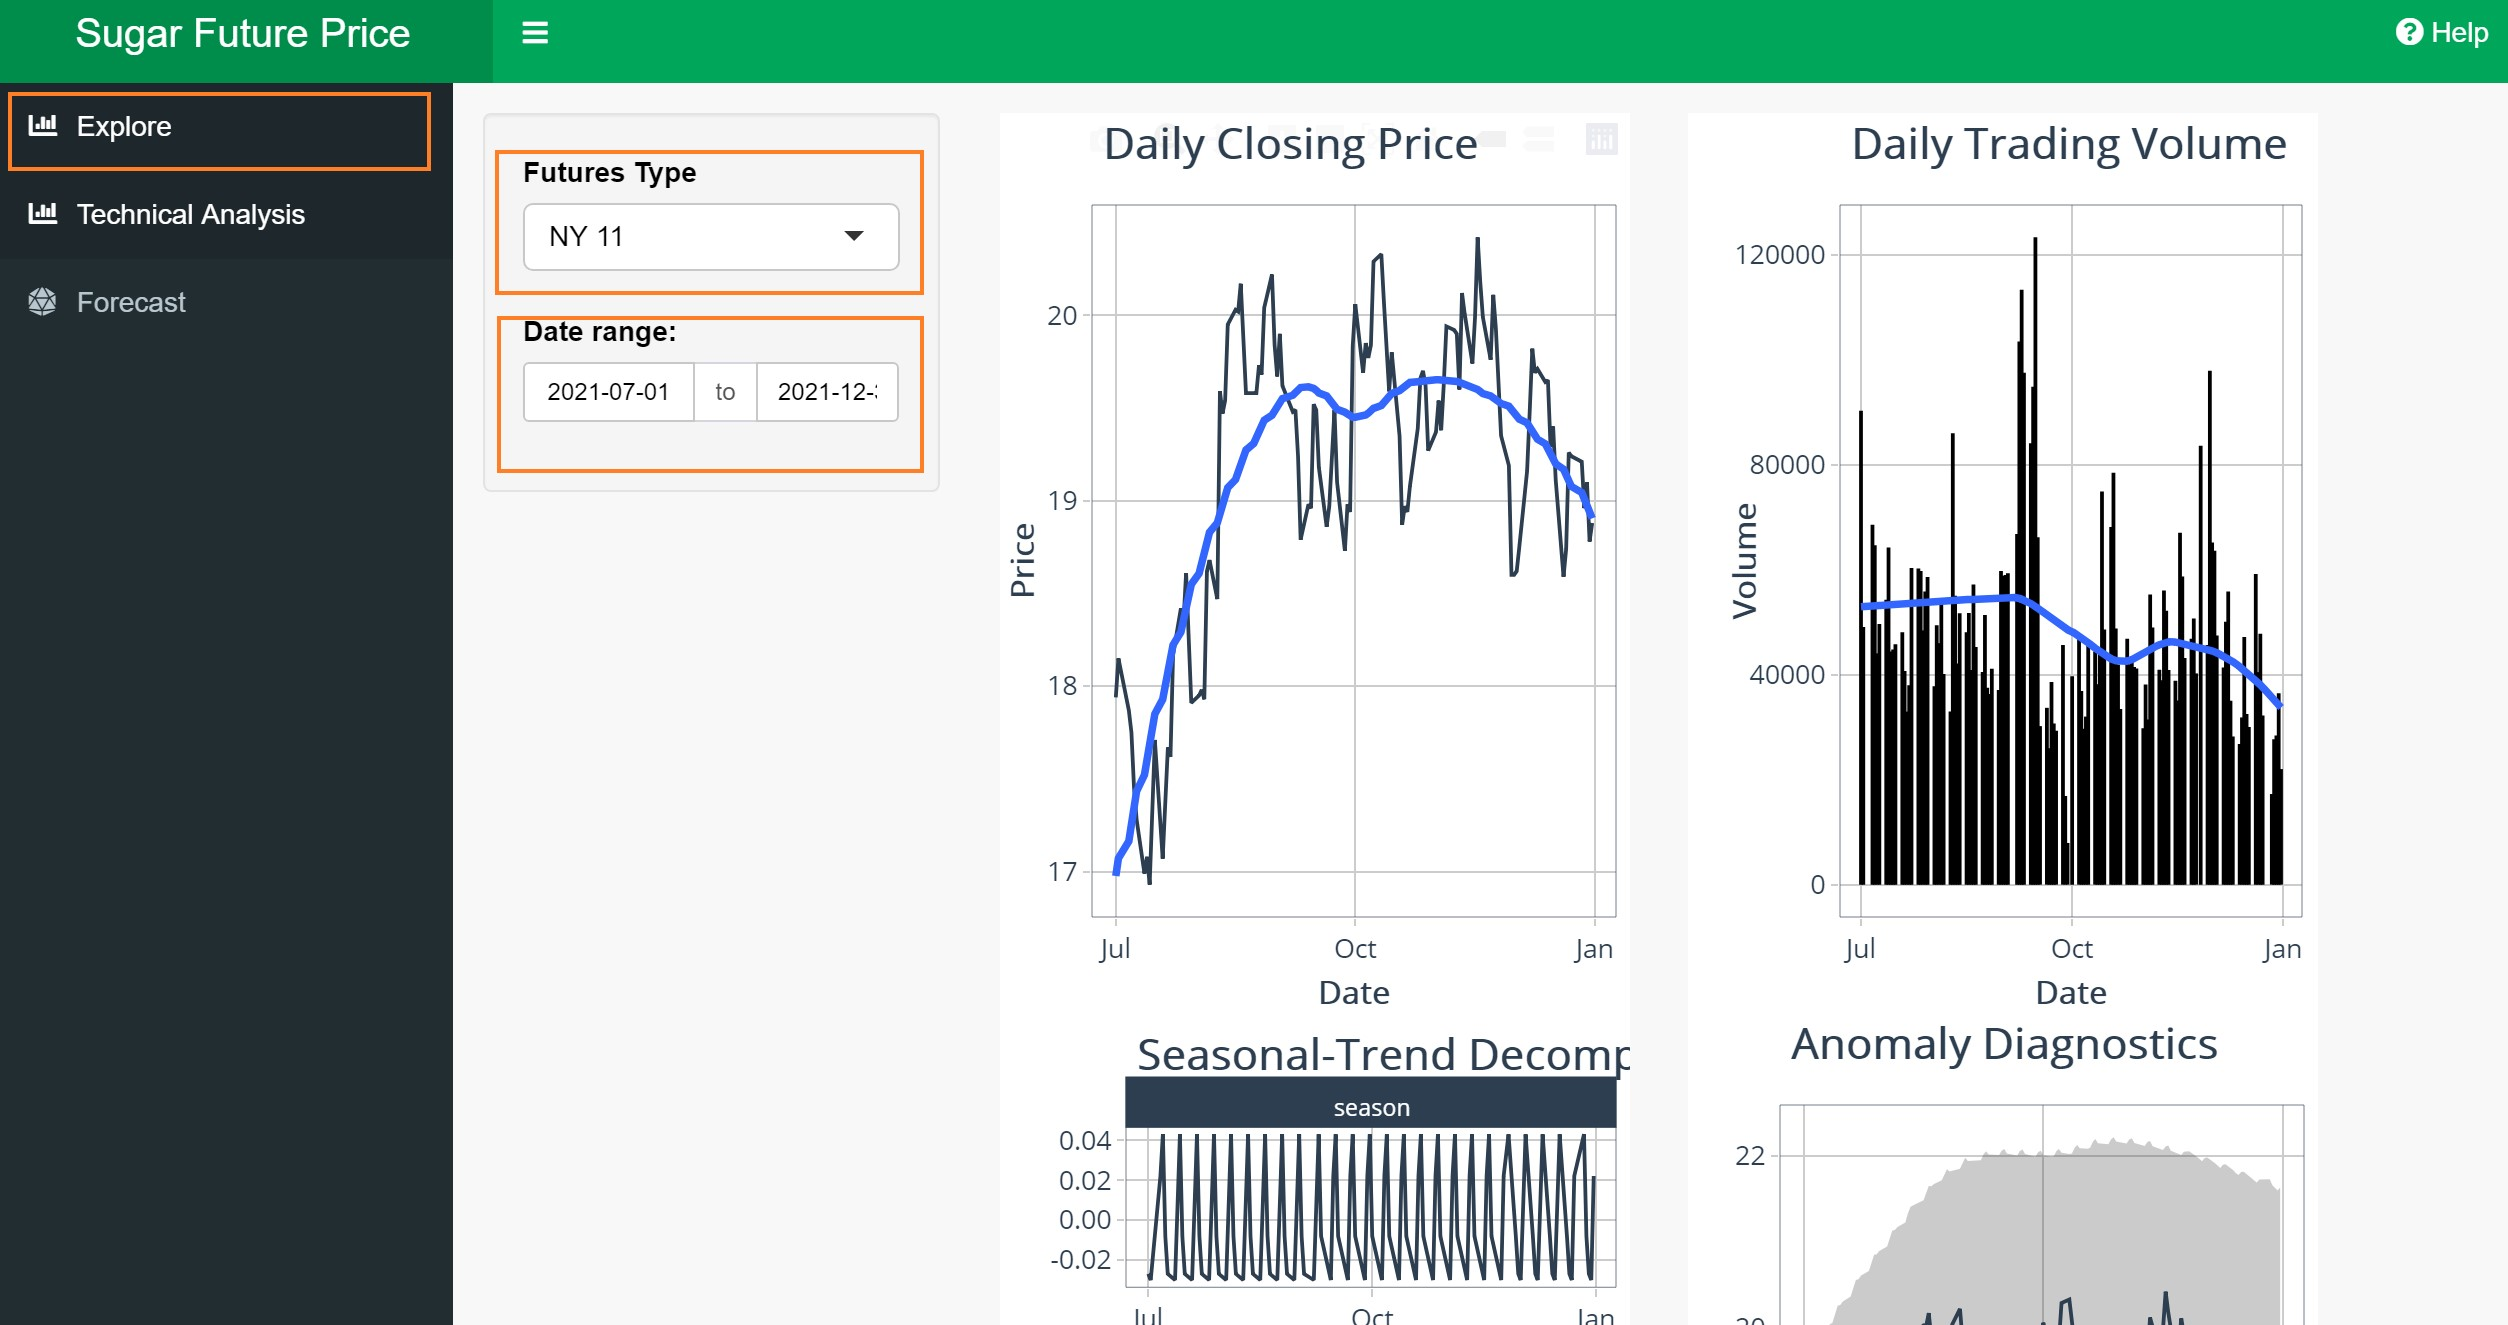
\includegraphics[width=1\linewidth]{images/EDA} \end{center}

\begin{enumerate}
\def\labelenumi{\arabic{enumi})}
\setcounter{enumi}{2}
\tightlist
\item
  User can mouse over to look the price of the particular dot.
\end{enumerate}

\begin{center}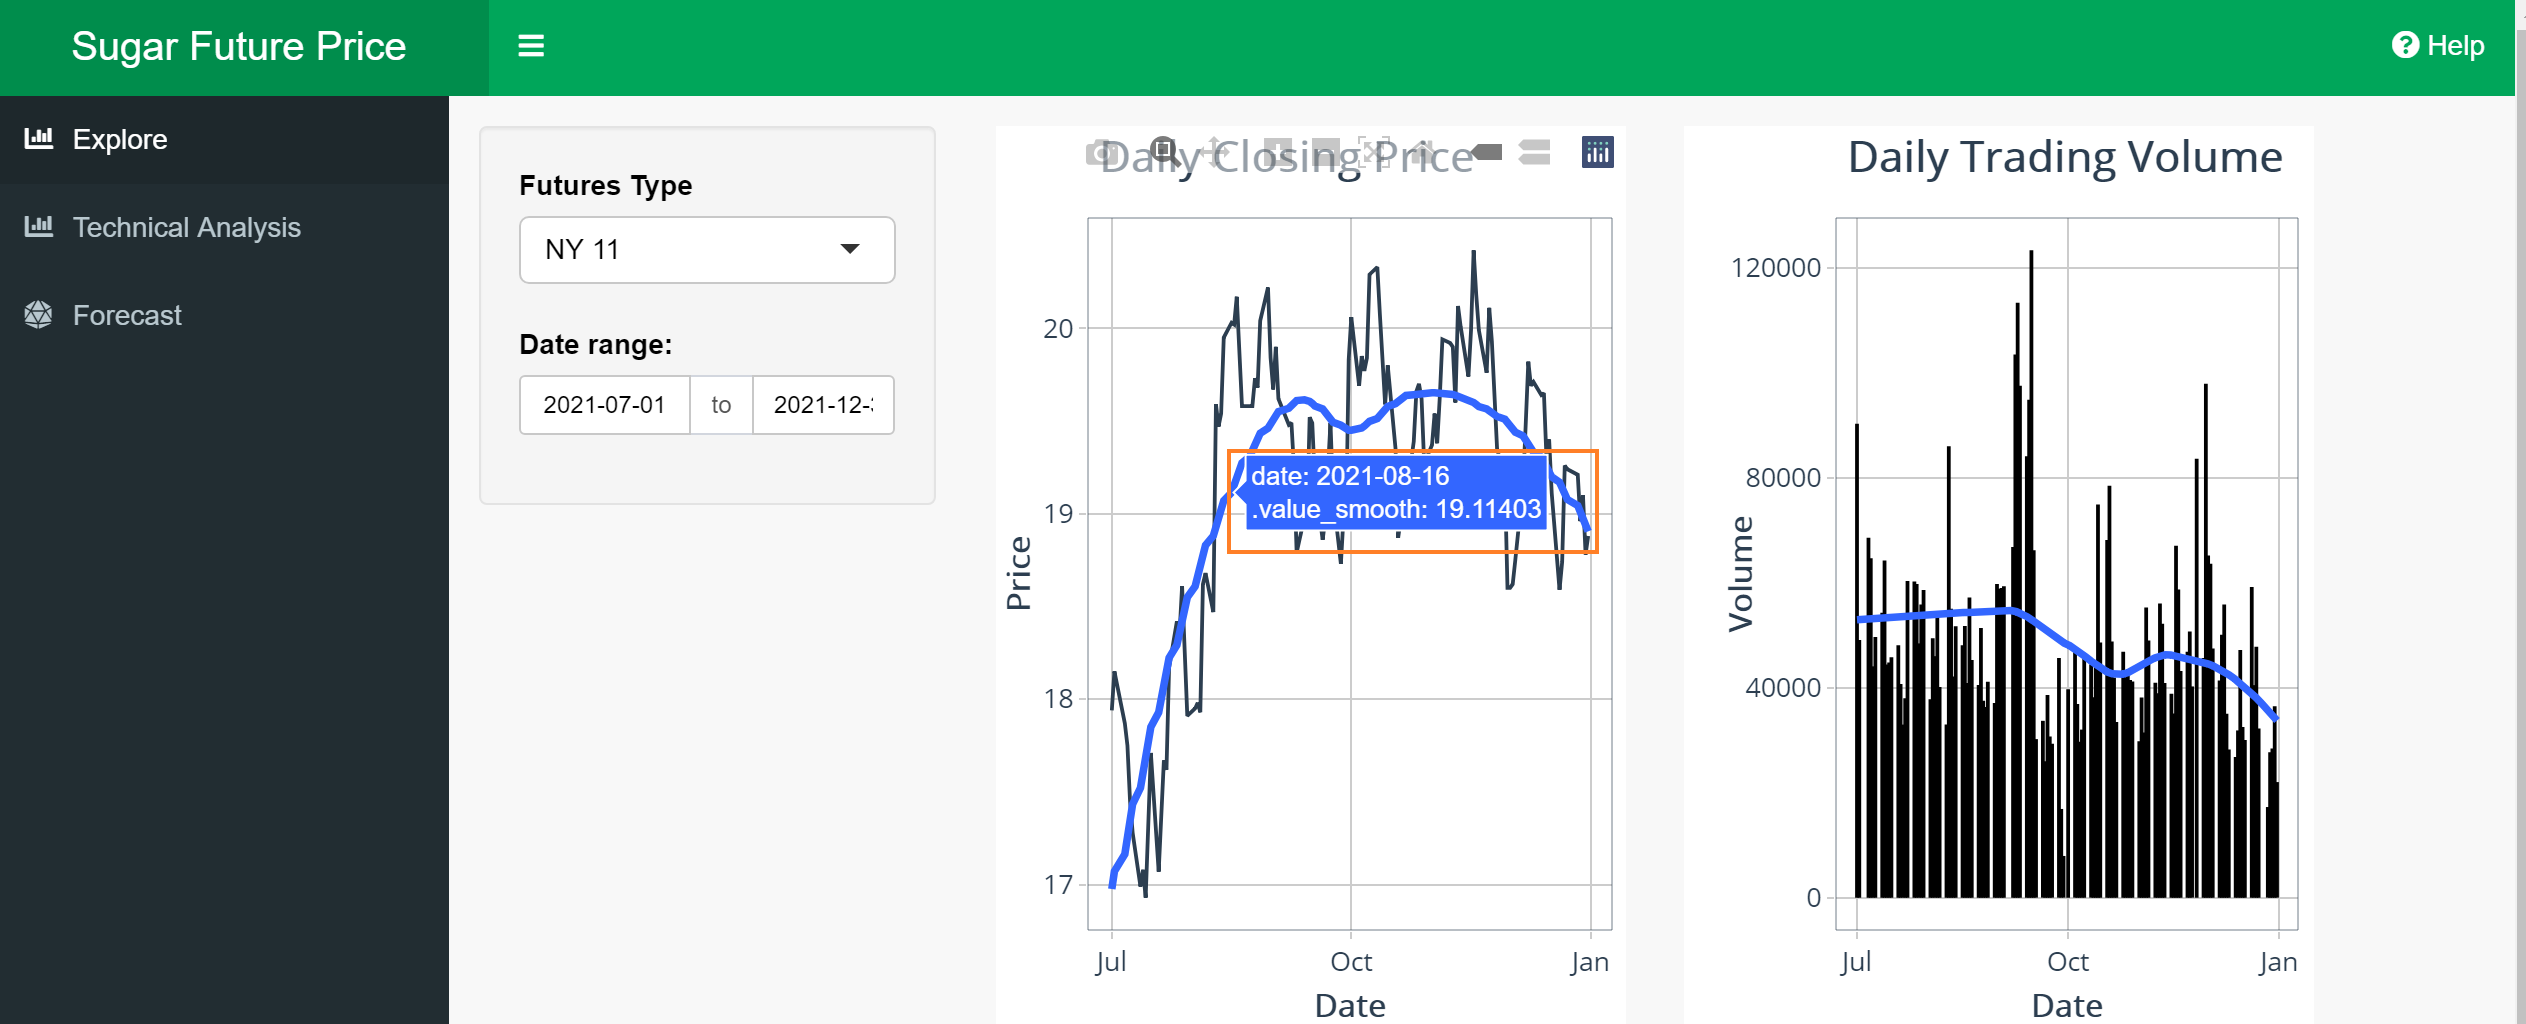
\includegraphics[width=1\linewidth]{images/EDA2} \end{center}

\begin{enumerate}
\def\labelenumi{\arabic{enumi})}
\setcounter{enumi}{3}
\tightlist
\item
  User can select the particular part to zoom in the visulisation.
\end{enumerate}

\begin{center}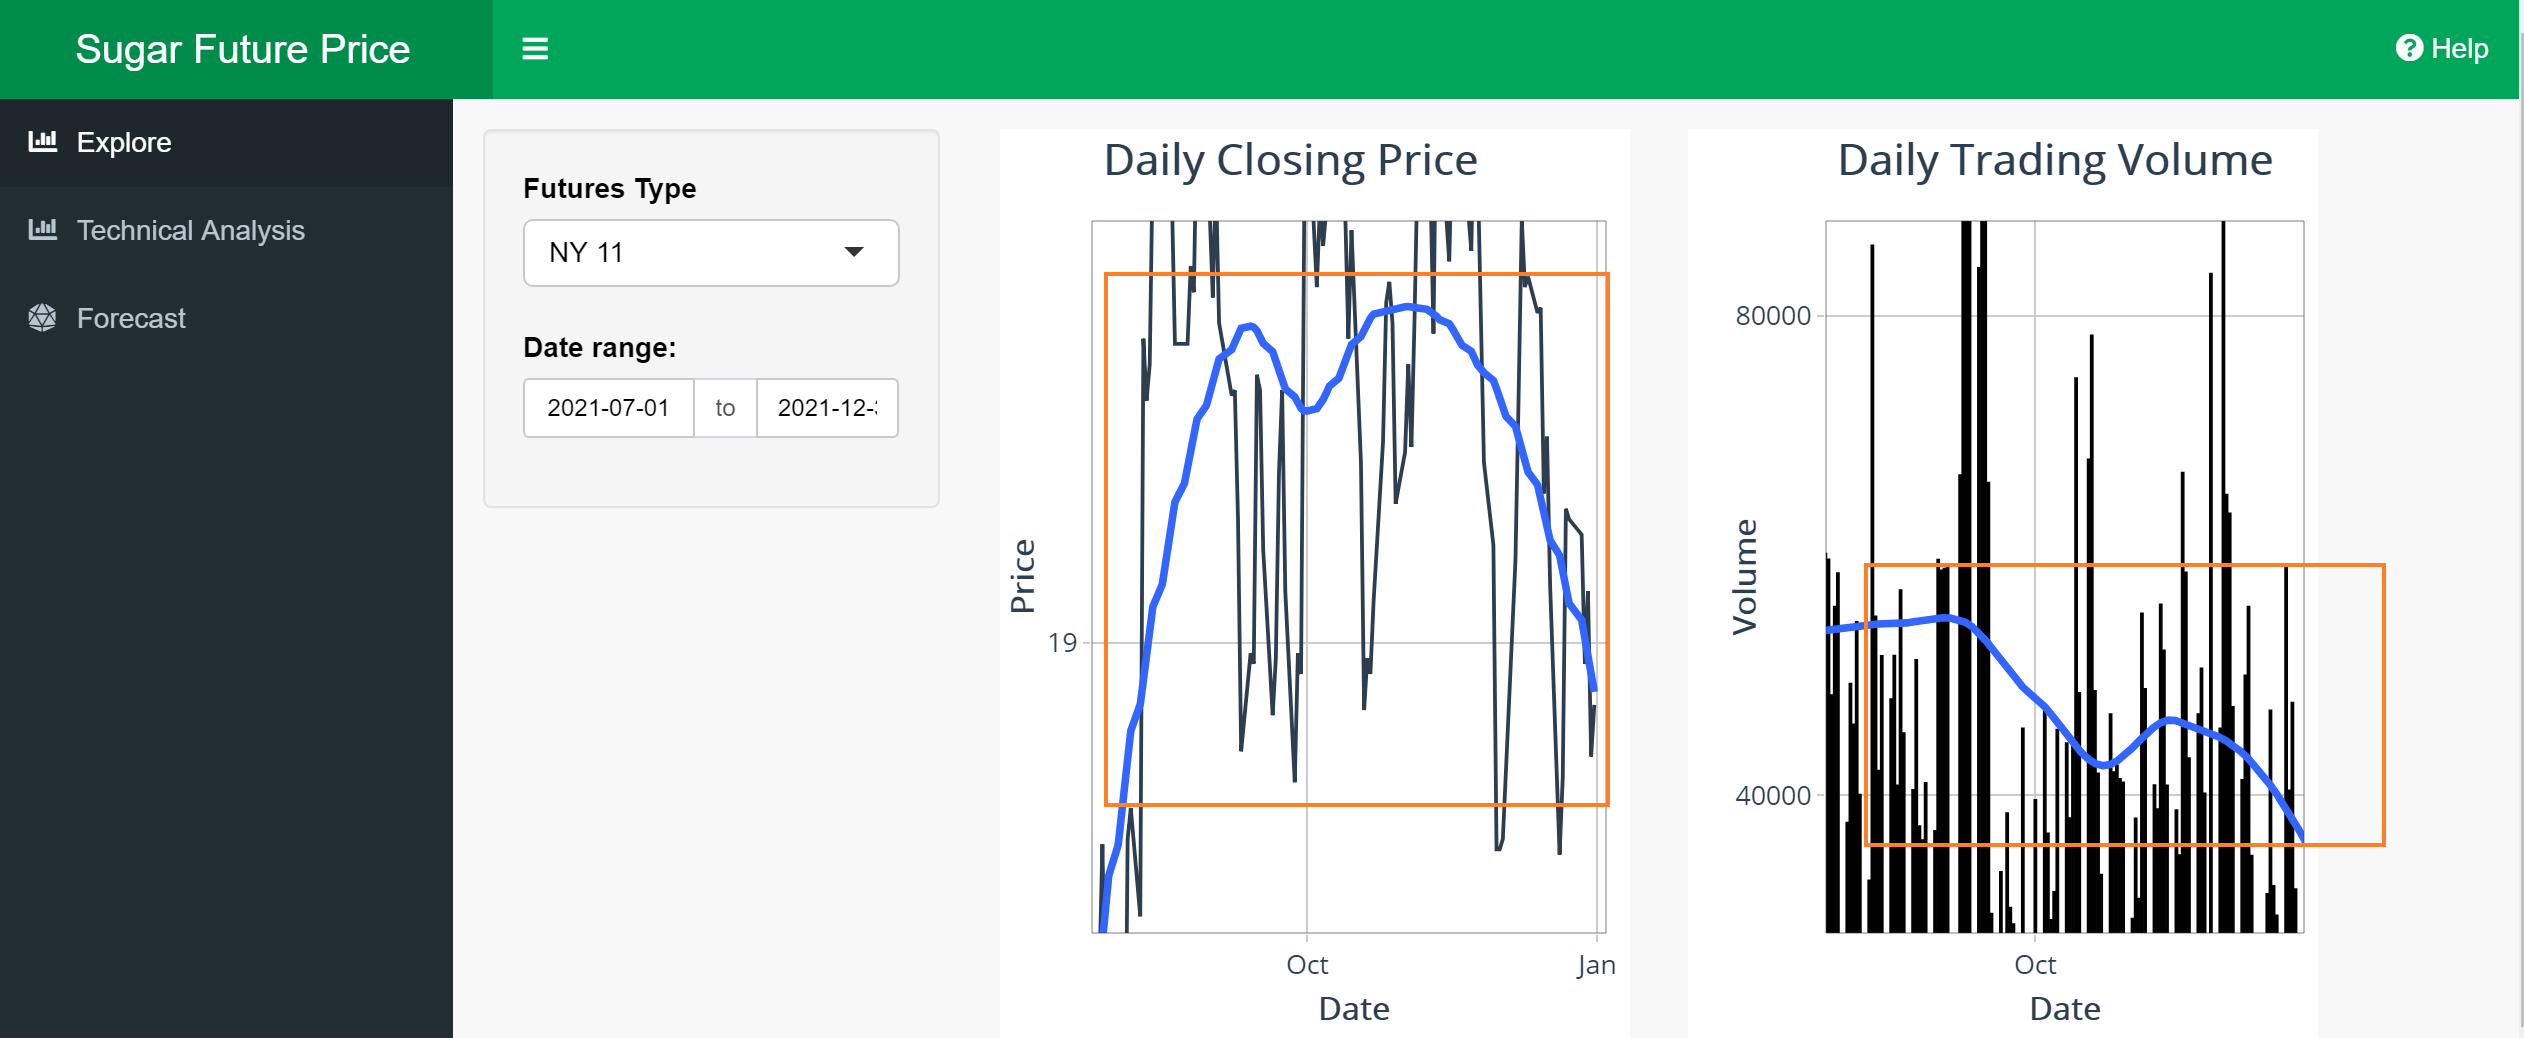
\includegraphics[width=1\linewidth]{images/EDA3} \end{center}

\hypertarget{technical-analysis}{%
\section{Technical Analysis}\label{technical-analysis}}

Except those steps are same as the explore part, it adds the chart type
button for users to choose. Users can follow the steps below:

\begin{enumerate}
\def\labelenumi{\arabic{enumi}.}
\tightlist
\item
  Click the tab and select the Date range for the analysis of your
  single future.
\end{enumerate}

\begin{center}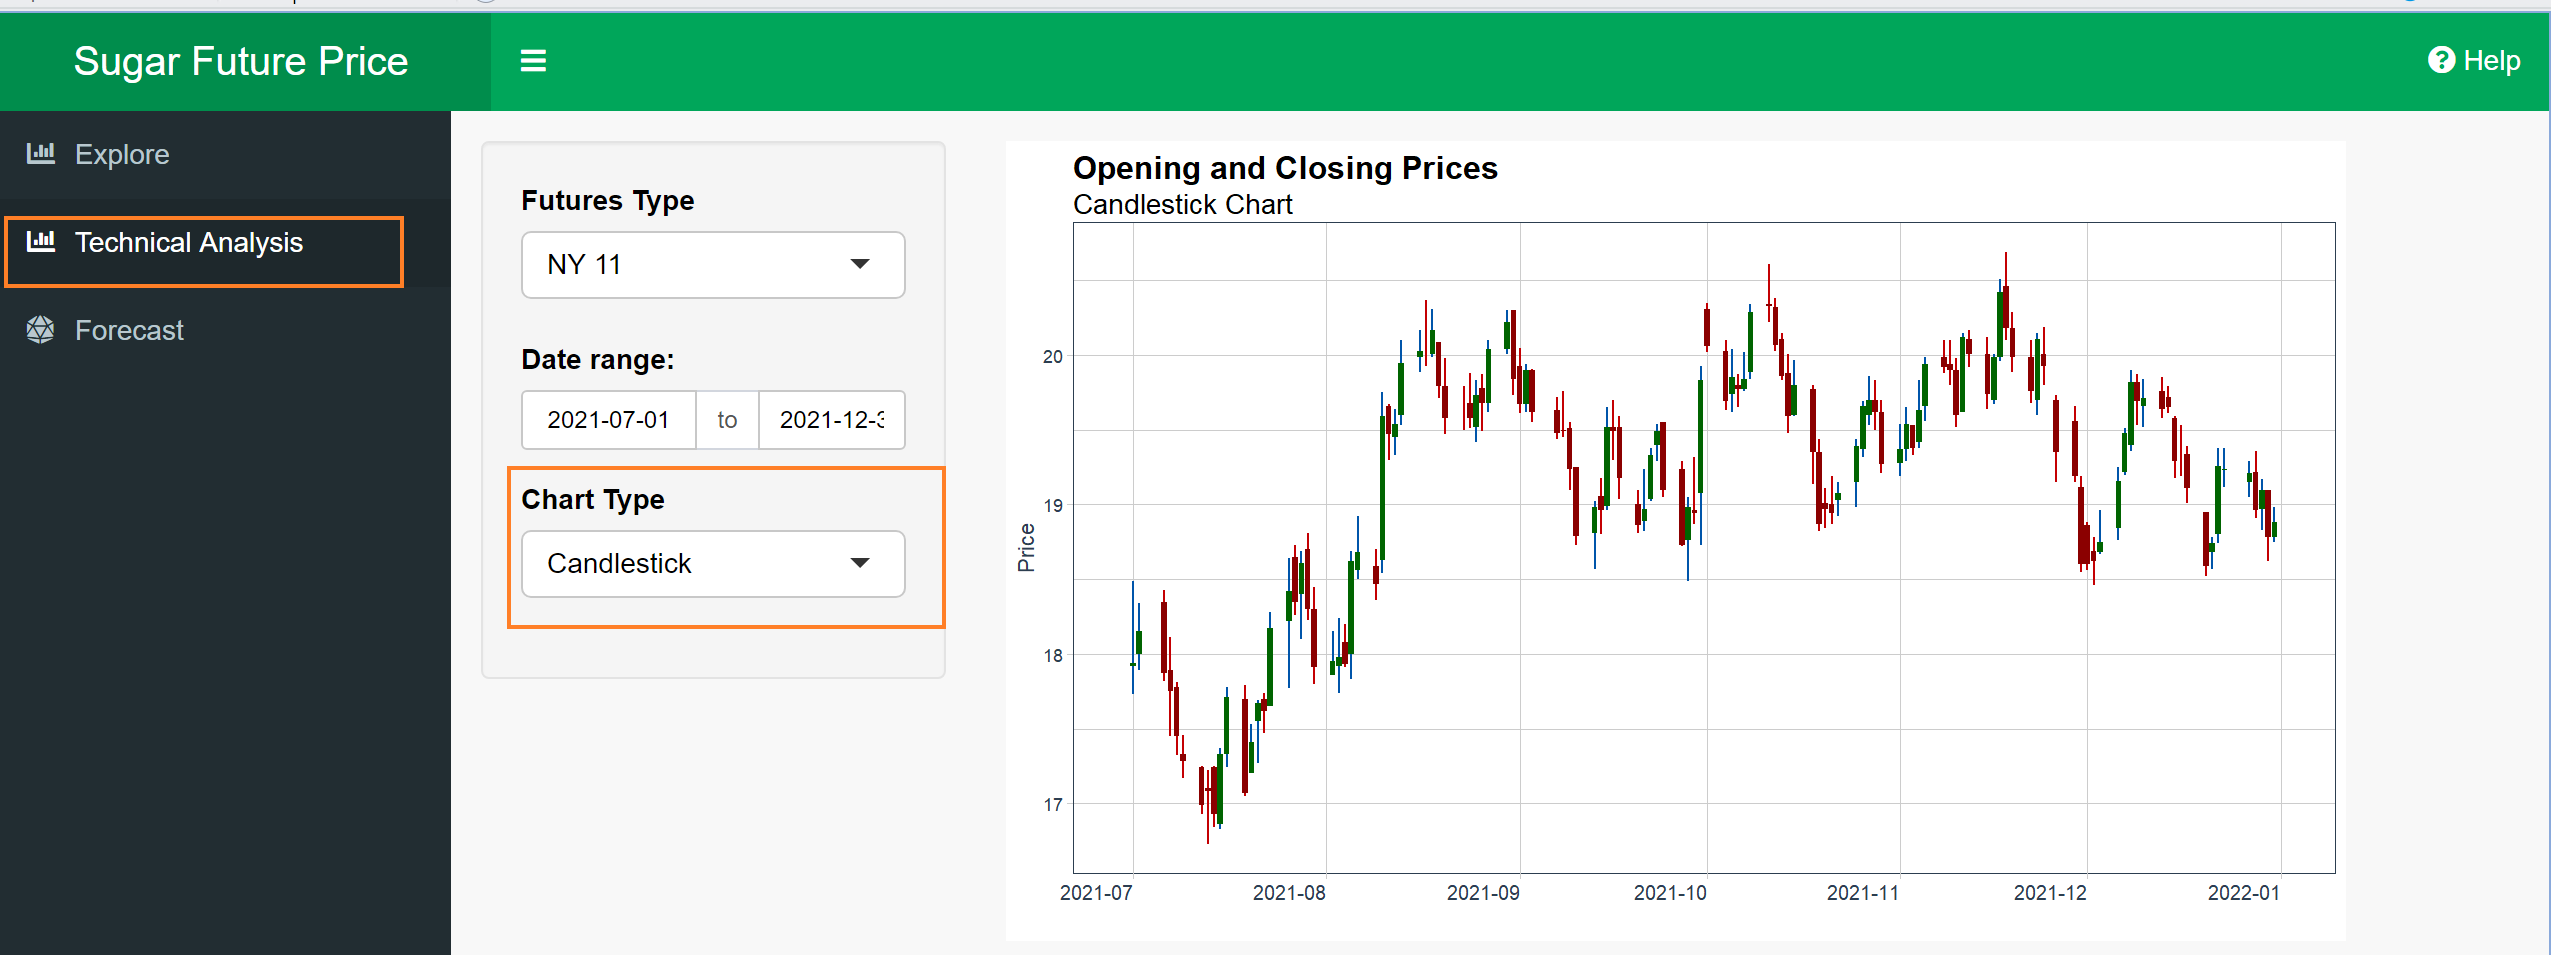
\includegraphics[width=1\linewidth]{images/for_1} \end{center}

\begin{enumerate}
\def\labelenumi{\arabic{enumi}.}
\setcounter{enumi}{1}
\item
  Select the type of chart you want to view by clicking the drop-down
  menu. The available options are:

  \begin{enumerate}
  \def\labelenumii{\alph{enumii}.}
  \item
    Candlestick Chart ¨C which will show the daily opening and closing
    prices for the future

    \begin{enumerate}
    \def\labelenumiii{\roman{enumiii}.}
    \item
      Red Bar means the stock closed lower, then when it opened
    \item
      Green Bar means the stock closed higher, then when it opened
    \end{enumerate}
  \end{enumerate}
\end{enumerate}

\begin{center}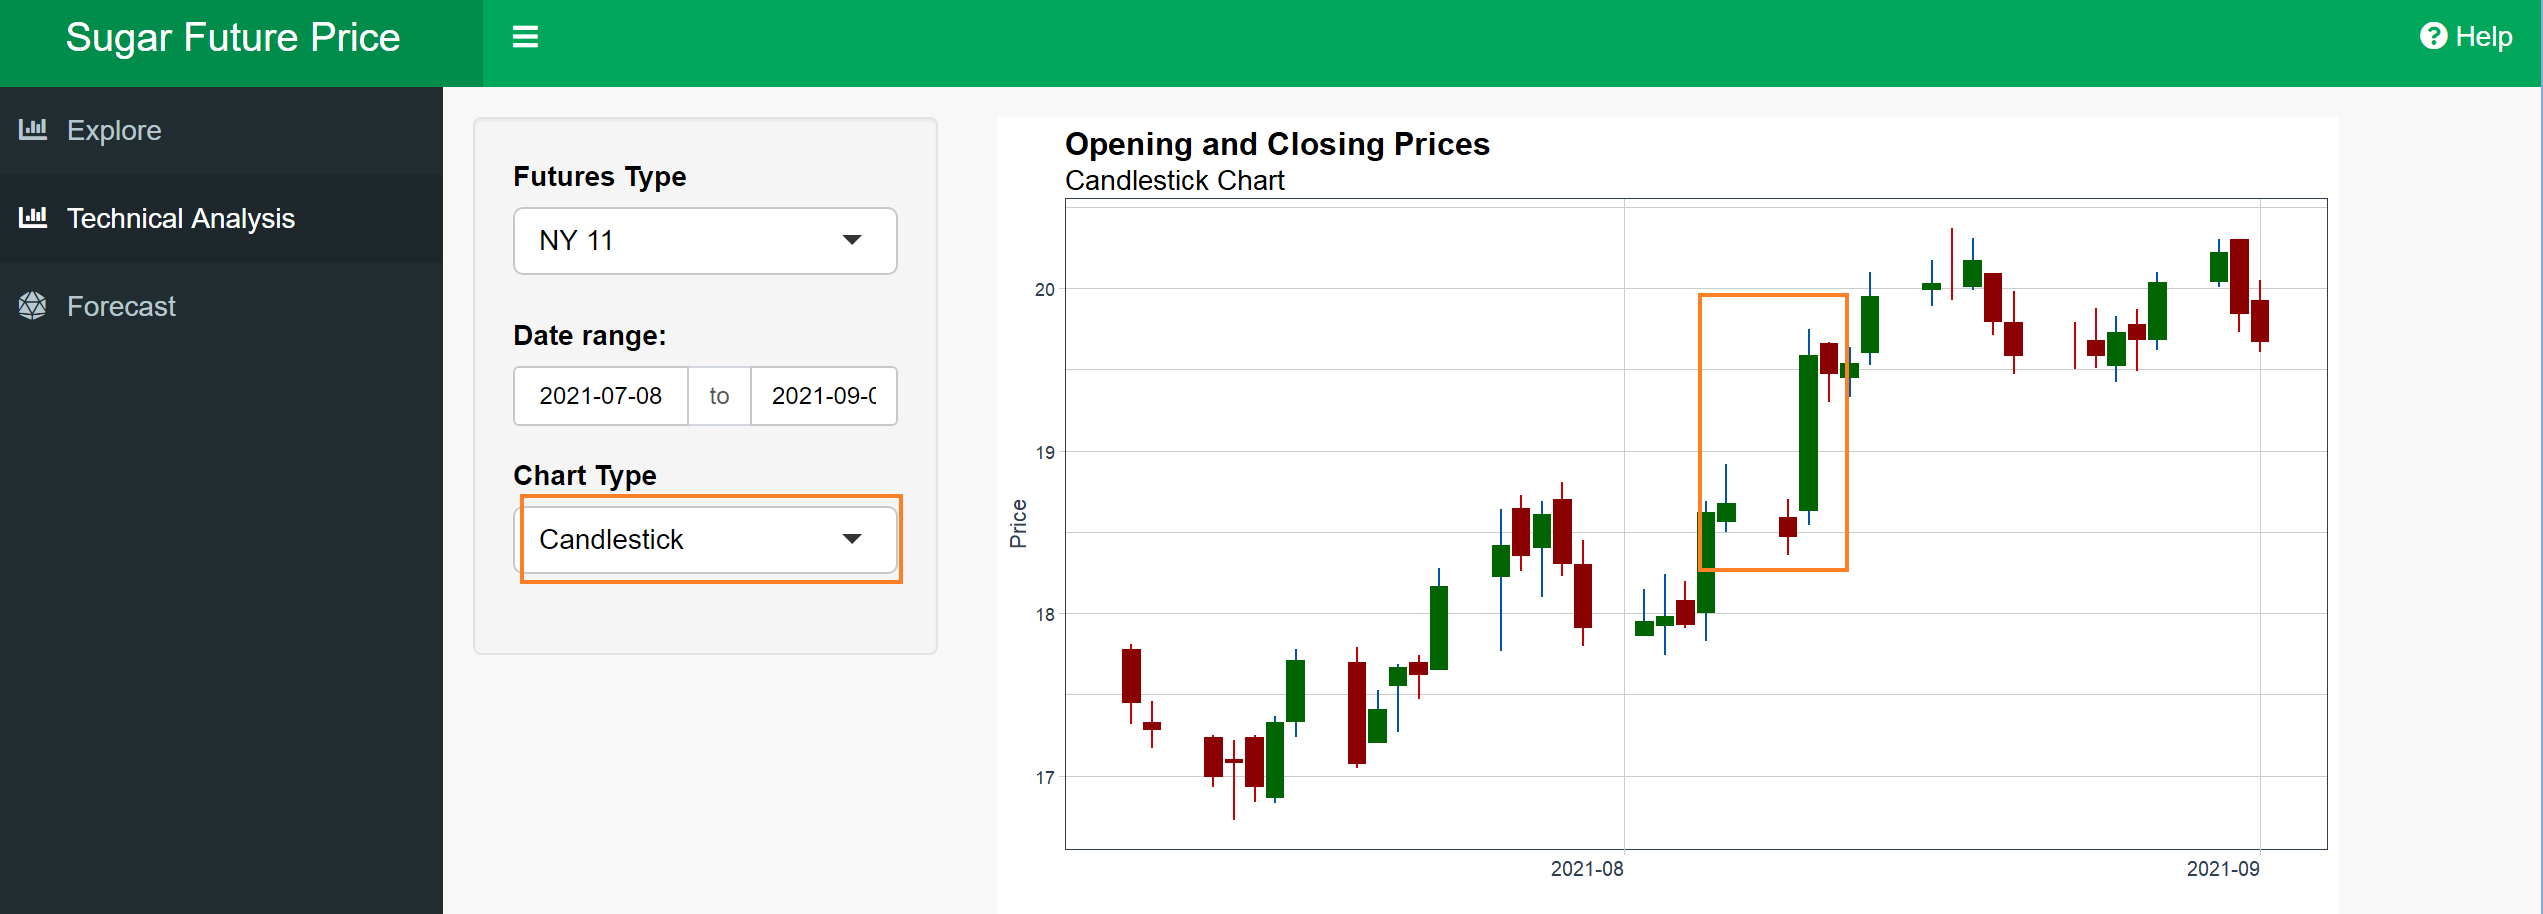
\includegraphics[width=1\linewidth]{images/TA_1} \end{center}

\begin{verbatim}
f. Averages ¨C Simple Moving Average (20 day and 50 day), overlayed with the candlestick chart 
\end{verbatim}

\begin{center}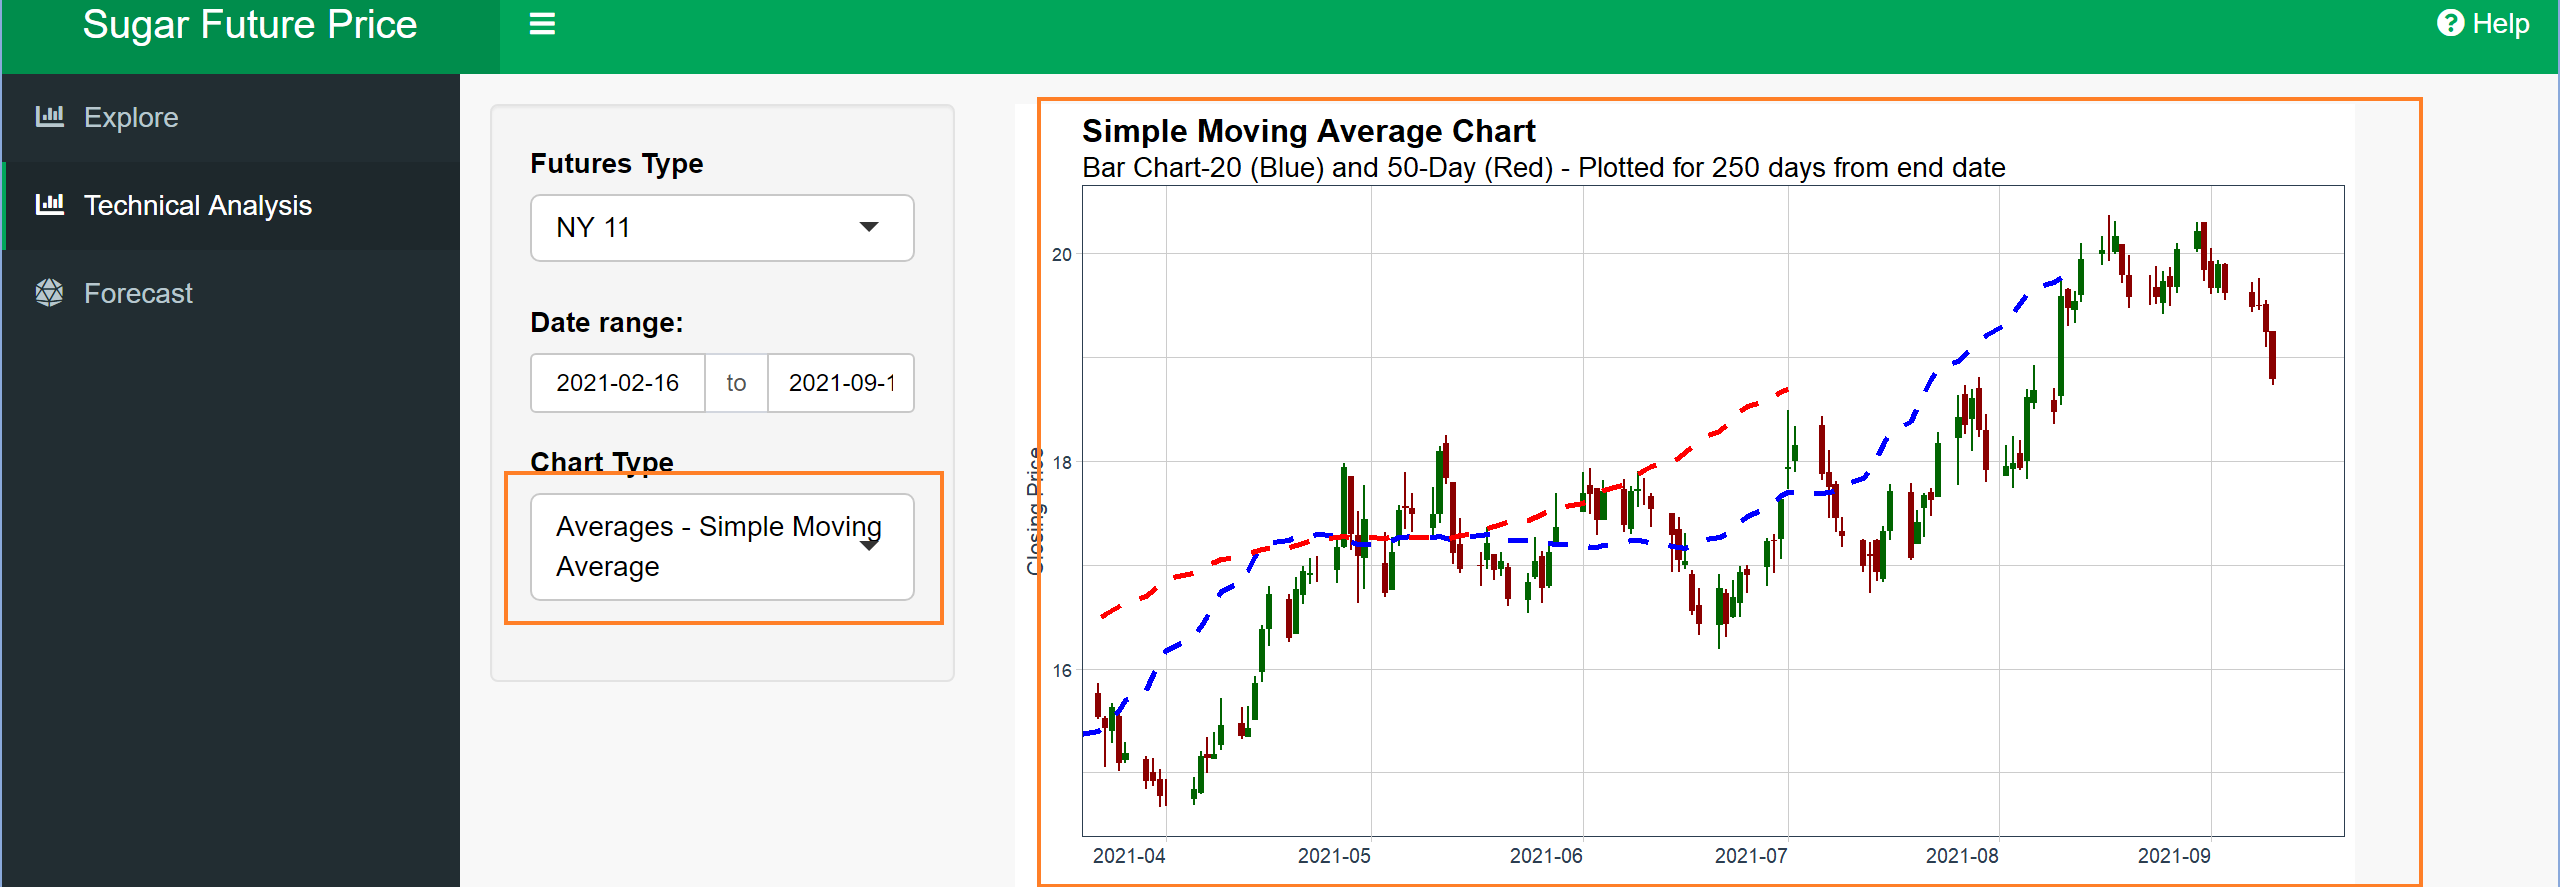
\includegraphics[width=1\linewidth]{images/TA_2} \end{center}

\begin{verbatim}
h. Averages ¨C Expoential Moving Average ( 20 day and 50 day ), overlayed with the candlestick chart 
\end{verbatim}

\begin{center}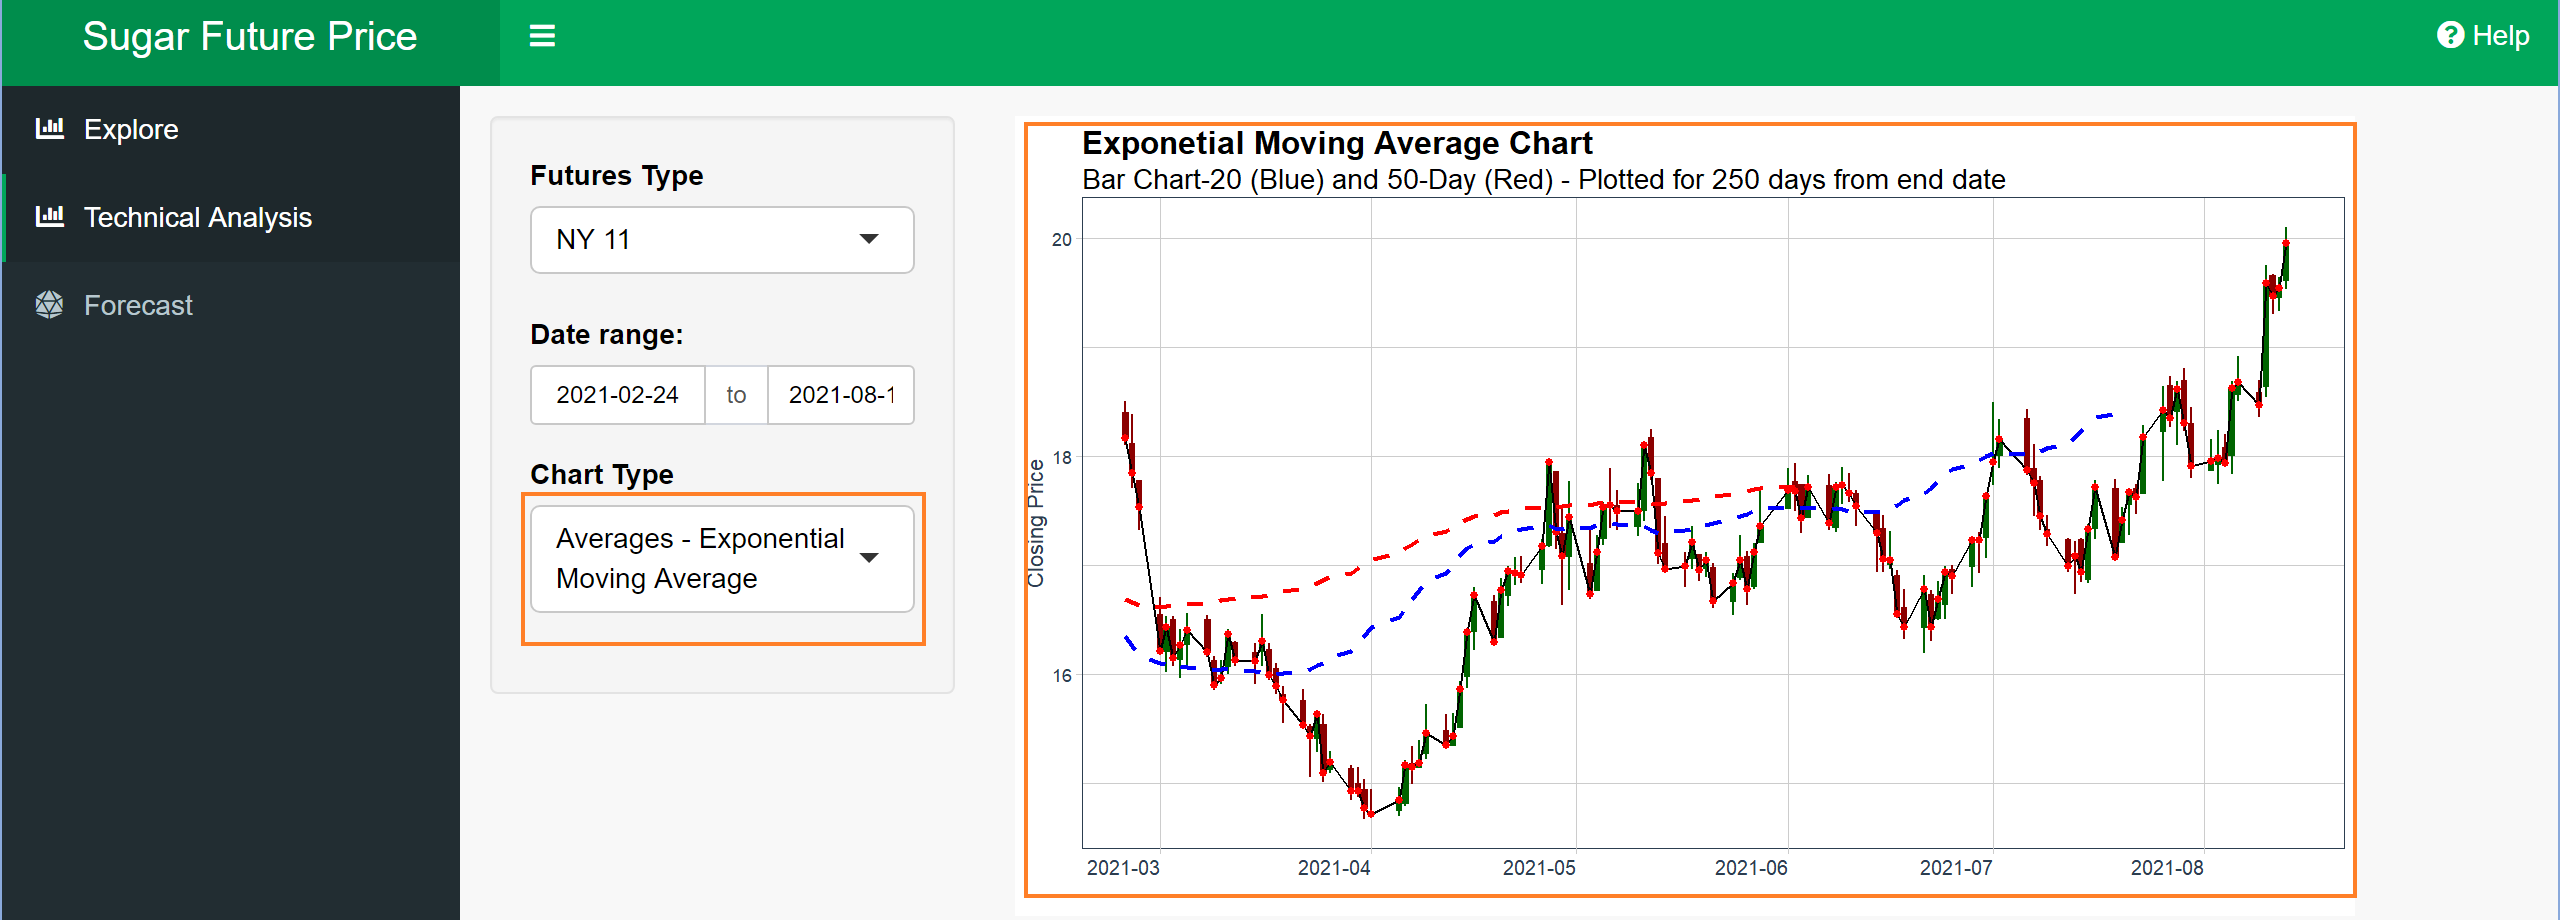
\includegraphics[width=1\linewidth]{images/TA_3} \end{center}

\begin{verbatim}
g. Averages ¨C Double Expoential Moving Average (20 day and 50 day), overlayed with the candlestick chart 
\end{verbatim}

\begin{center}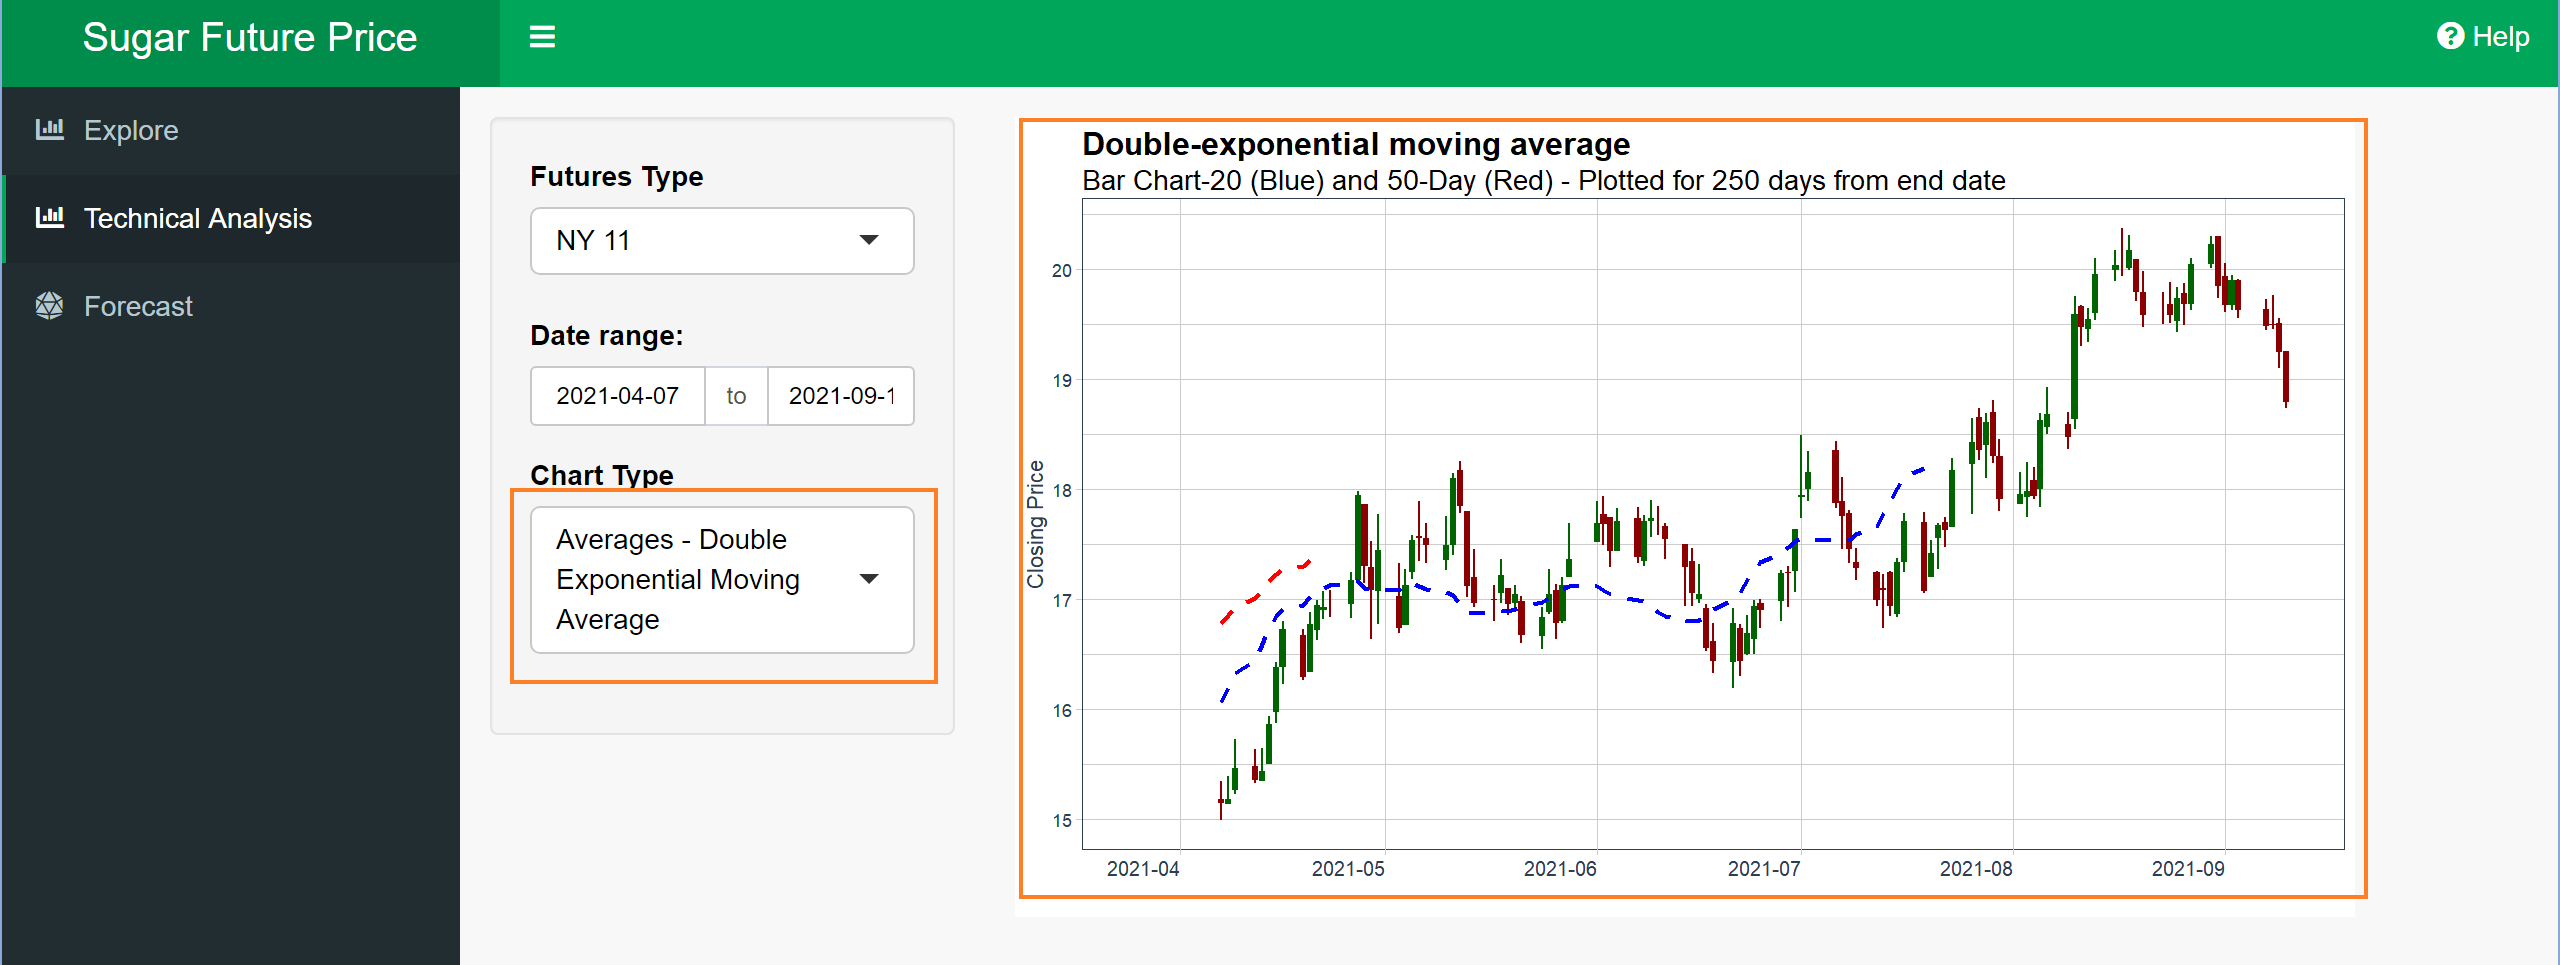
\includegraphics[width=1\linewidth]{images/TA_4} \end{center}

\begin{enumerate}
\def\labelenumi{\alph{enumi}.}
\setcounter{enumi}{7}
\tightlist
\item
  Averages ¨C Elastic Volume-Weighted Moving Average (20 day and 50
  day), overlayed with the candlestick chart
\end{enumerate}

\begin{center}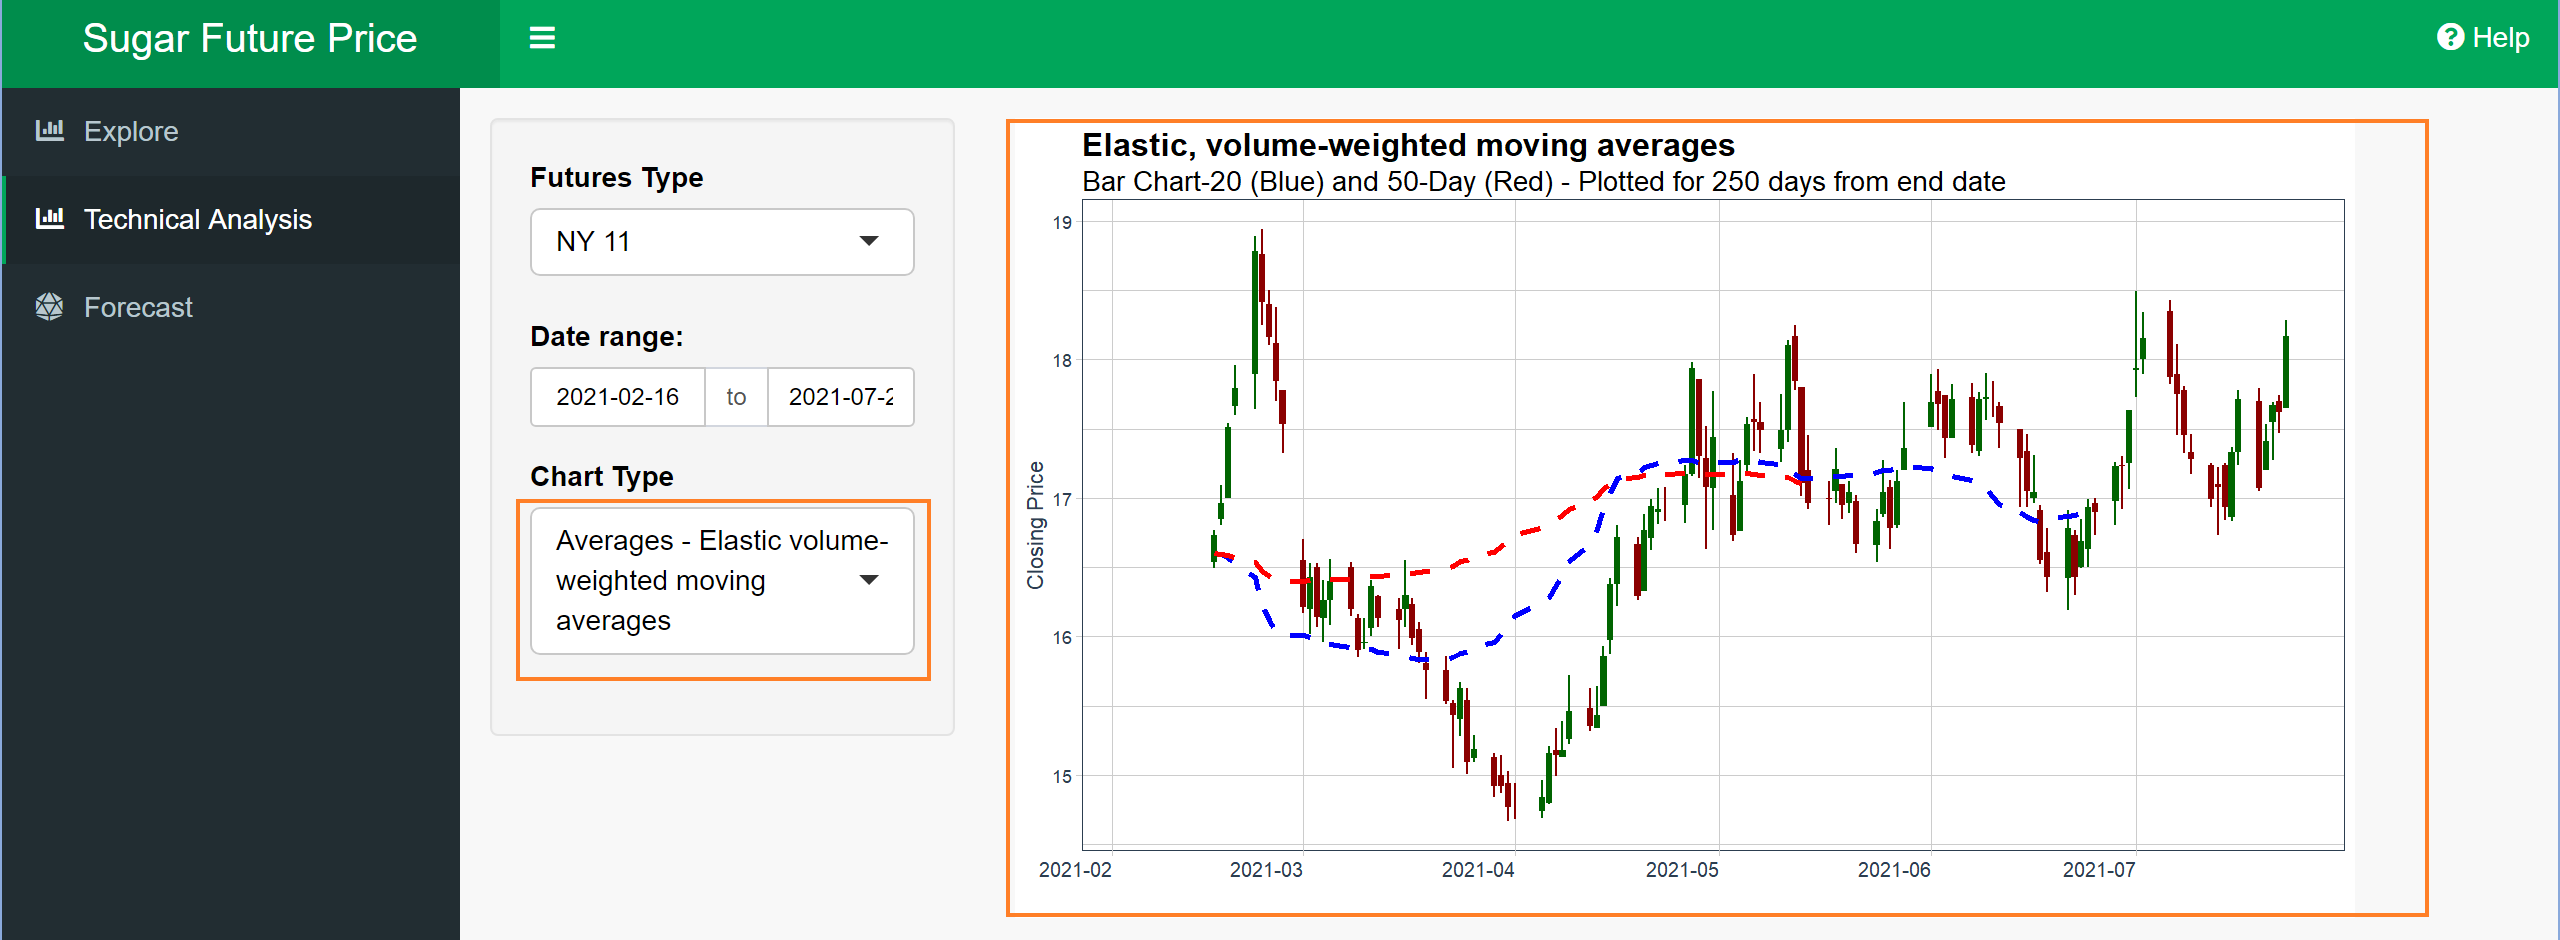
\includegraphics[width=1\linewidth]{images/TA_5} \end{center}

\begin{verbatim}
 i. Simple Moving Average with Bollinger Bands 
\end{verbatim}

\begin{center}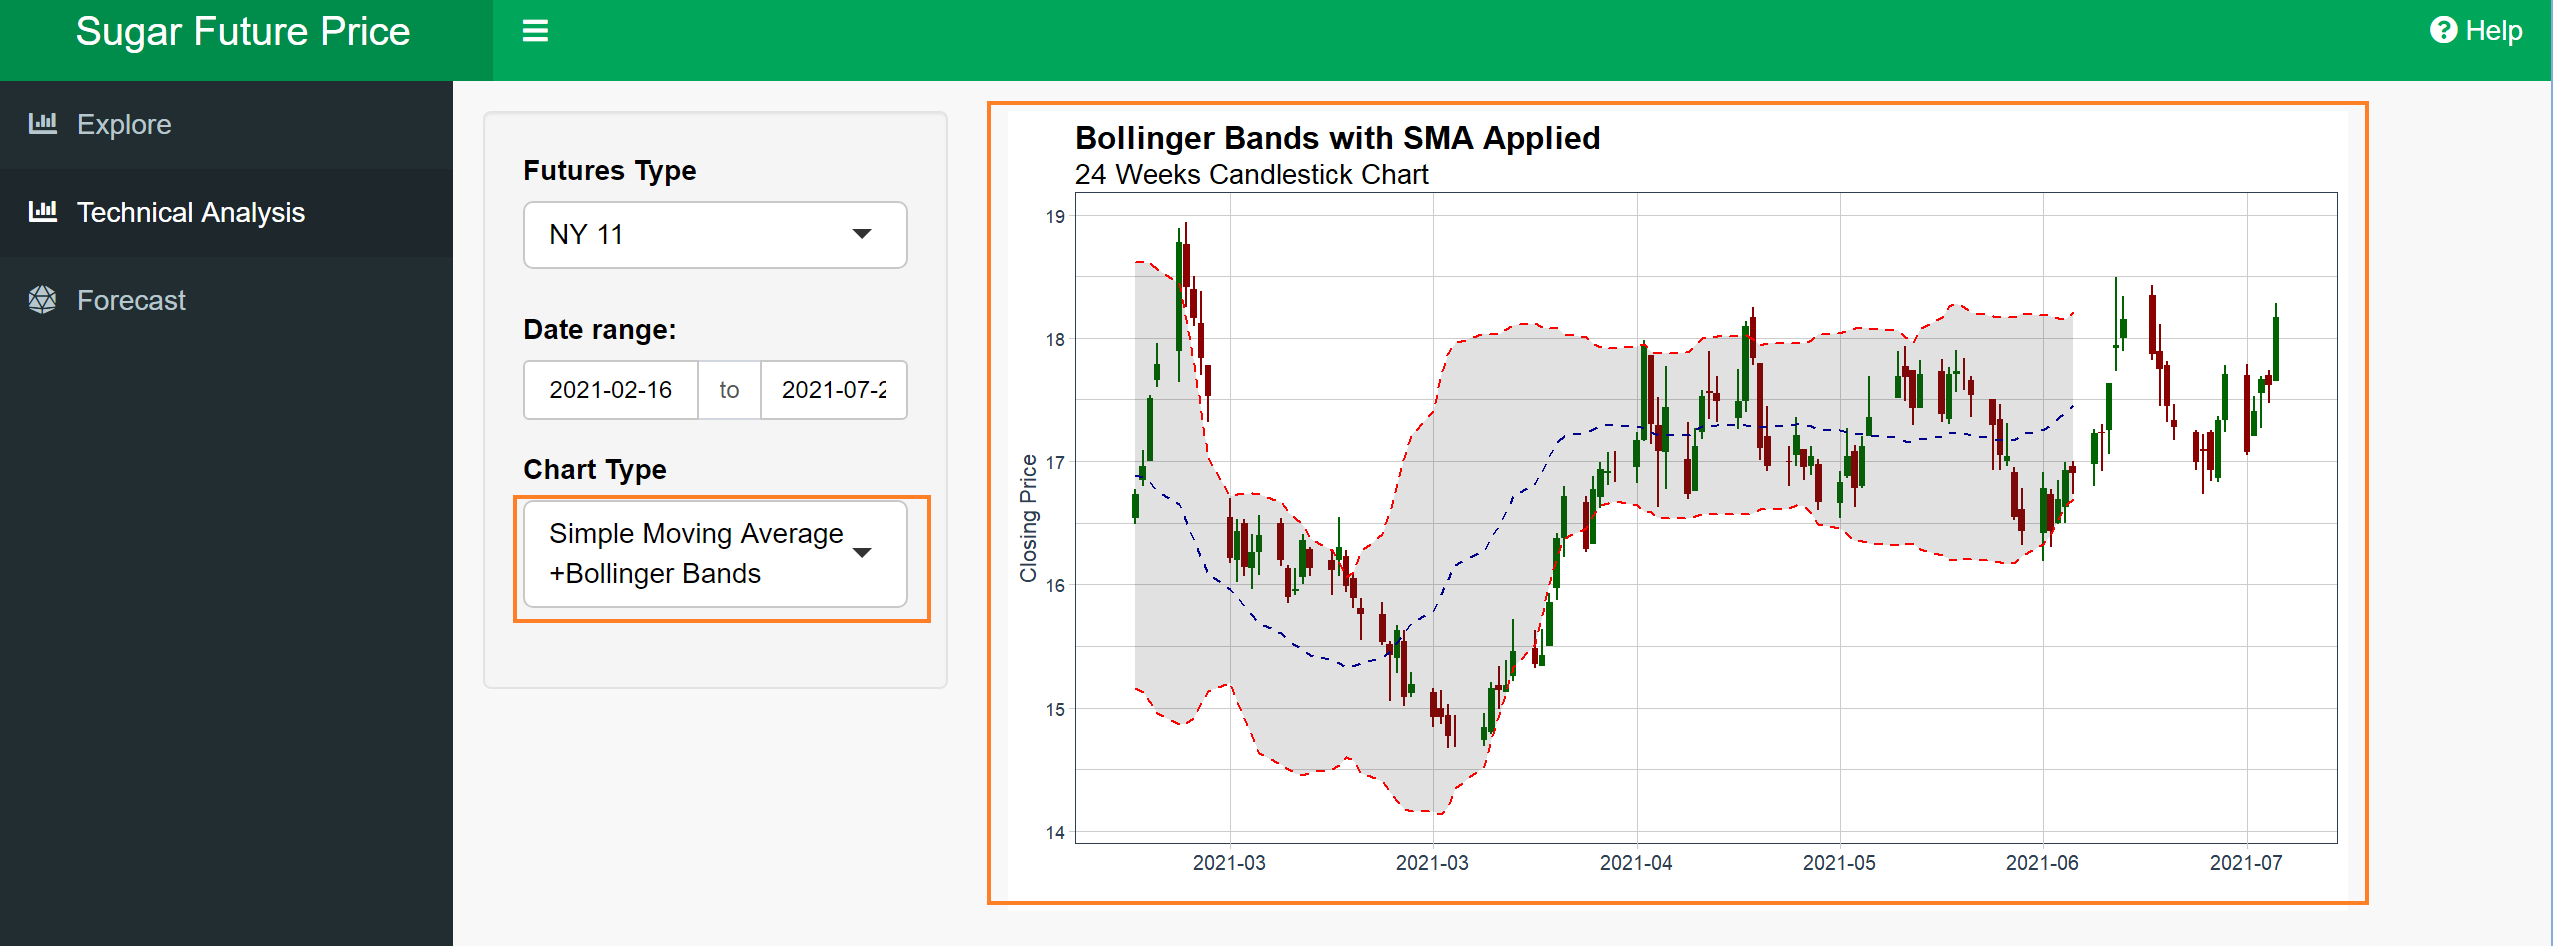
\includegraphics[width=1\linewidth]{images/TA_6} \end{center}

~~~~~~As the actual mathematical and technical definition of the
averages are beyond of the scope of this user guide, please visit this
link to understand what they mean before analyzing the chart:
\href{https://business-science.github.io/tidyquant/reference/geom_ma.html}{Plot
moving averages}

\# Forecast

\hypertarget{general}{%
\section{General}\label{general}}

At the right of the name of shiny app, there is an icon to hide the
three main parts names if the users don¡¯t want to see. And at the top
right of the green bar is a button for users guide to seek help.

\begin{center}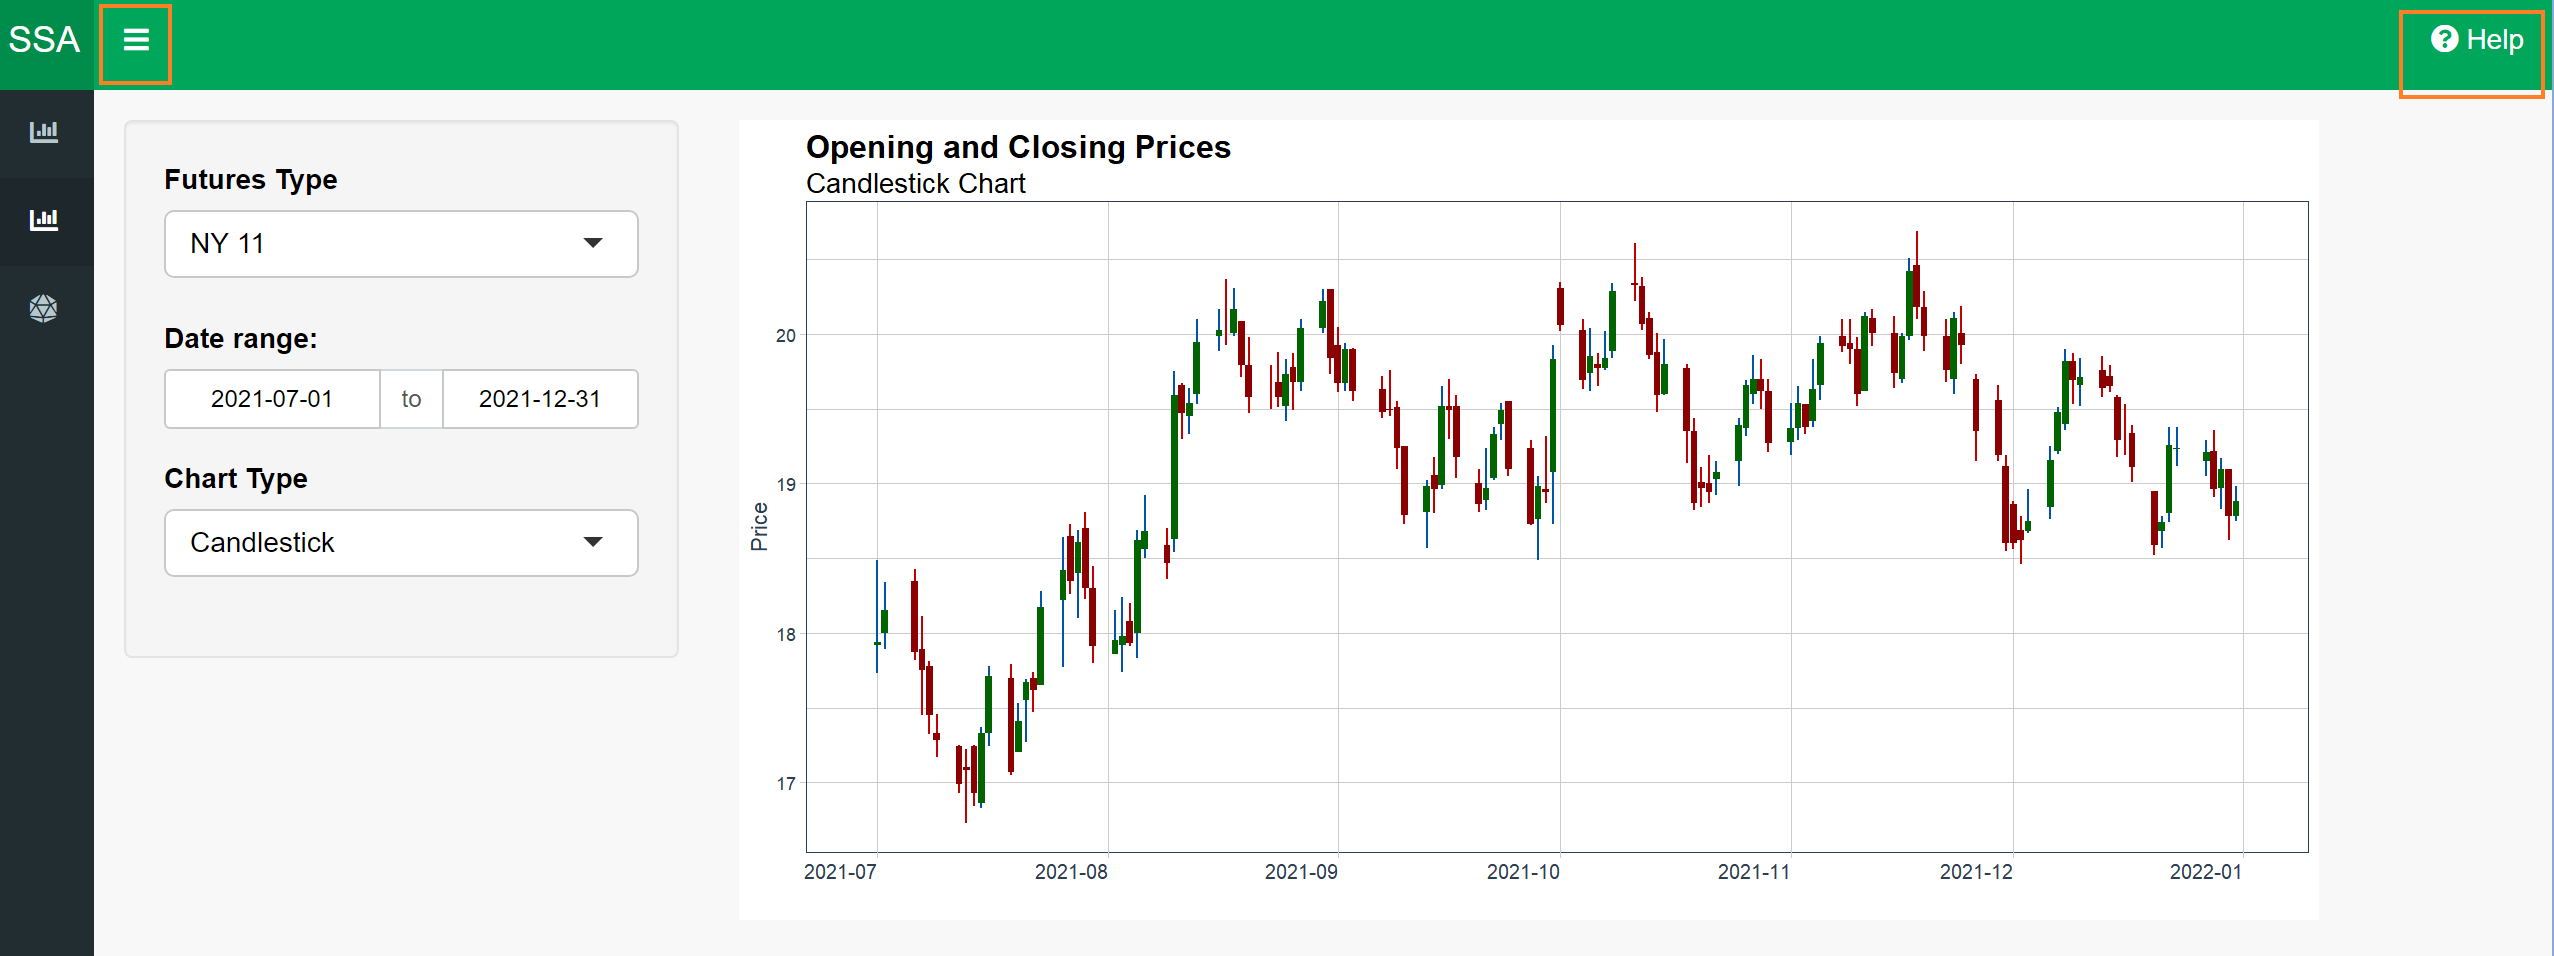
\includegraphics[width=1\linewidth]{images/1} \end{center}

\end{document}
